% \section{Appendix}
\subsection{Example SVAs}
\label{subsec:Example-SVAs}
Across all $10$ examples in Table~\ref{tab:example_svas}, the SVAs generated by our customized RAG framework pass the functionality verification, meaning they accurately implement the property. In contrast, the SVAs generated by GPT-4o-mini exhibit functionality mismatches in every case.  Common issues include incorrect usage of temporal operators (such as overlapping implication operator \texttt{|->} and non-overlapping implications operator \texttt{|=>}), improper handling of past signal values, and failure to accurately capture the specified clock-cycle timing relationships.
\begin{table*}[ht]
    \centering
    \caption{Examples of SVAs generated by GPT-4o-mini and RAGSVAG.}
    \label{tab:example_svas}
    \begin{tabular}{|c|c|p{3.8cm}|p{5.4cm}|p{5.4cm}|}
        \hline
        \textbf{Design} & \textbf{Lines} & \textbf{Natural Language Explanation} & \textbf{GPT-4o-mini SVA} & \textbf{RAGSVAG SVA} \\
        \hline
        ff & $10$ & When enable signal is set (1), output equals input from previous cycle in next cycle. & \texttt{assert property (@(posedge clk) disable iff (rst) (en == 1'b1 |=> out == in[1]));} & \texttt{assert property (@(posedge clk) disable iff (rst) (en |=> (out == \$past(in))));} \\
        \hline
        PWM & $18$ & Eventually, the inversion of the output becomes true. & \texttt{assert property (@(posedge clk) (pulse |-> eventually (!pulse)));} & \texttt{assert property (@(posedge clk) (s\_eventually (!pulse)));}\\
        \hline
        register & $20$ & When enable reset (0), output equals last output in next cycle. & \texttt{assert property (@(posedge clk) disable iff (rst) (en == 0 |-> out == out[1]));} & \texttt{assert property (@(posedge clk) disable iff (rst) (en == 0 |=> (out == \$past(out))));} \\
        \hline
        simple\_req\_ack & $31$ & When request signal is detected to have a rising edge, then after a delay of $2$ clock cycles the acknowledge signal is detected to have a rising edge. & \texttt{assert property (@(posedge clk) disable iff(!rst\_n) (req\_ff in \{1'b0, 1'b1\} during [2] |=> (ack\_ff == 1'b1)));} & \texttt{assert property (@(posedge clk) disable iff(!rst\_n) (\$rose(req) |=> \#\#2 \$rose(ack)));} \\
        \hline
        or1200\_if & $194$ & When pipeline flush signal is reset ($0$) and save instruction condition is true, then saved flag equals 1 in the next clock cycle. & \texttt{assert property (@(posedge clk) disable iff (rst) (if\_flushpipe == 0 \&\& save\_insn |-> saved));} & \texttt{assert property (@(posedge clk) disable iff (rst) (if\_flushpipe == 0 \&\& save\_insn |=> (saved == 1)));} \\
        \hline
        arbiter & $231$ & When the first bit of grant output is asserted and in the previous clock cycle the arbitration type selector signal was equal to $0$, then the first bit of request input signal from the previous clock cycle must be asserted in the current clock cycle. & \texttt{assert property (@(posedge clk) disable iff (\textasciitilde rst\_n) (gnt[0] \&\& arb\_type == 0 |-> req[0]));} & \texttt{assert property (@(posedge clk) disable iff (\textasciitilde rst\_n) ((gnt[0] \&\& \$past(arb\_type) == 0) |-> \$past(req[0])));} \\
        \hline
        a25\_wishbone & $447$ & When the wishbone bus state equals \texttt{WB\_BURST1} and the acknowledgement signal is asserted, then the wishbone bus state equals \texttt{WB\_BURST2} in the next clock cycle. & \texttt{assert property (@(posedge i\_clk) (wishbone\_st == WB\_BURST1 \&\& i\_wb\_ack |-> (wishbone\_st == WB\_BURST2)));} & \texttt{assert property (@(posedge i\_clk) ((wishbone\_st == WB\_BURST1 \&\& i\_wb\_ack) |=> (wishbone\_st == WB\_BURST2)));} \\
        \hline
        control\_unit & $602$ & When the signal that indicates the beginning of an AES operation equals 0, then the signal used to initialize the key generation process equals 0 in the current clock cycle. & \texttt{assert property (@(posedge clk) (start == 0 |=> key\_init == 0));} & \texttt{assert property (@(posedge clk) (start == 1'b0 |-> key\_init == 1'b0));} \\
        \hline
        or1200\_ctrl & $1225$ & When the freeze signal for the EX stage is reset ($0$) and either the freeze signal for the ID stage is set ($1$) or the pipeline flush signal for the EX stage is set ($1$), then the signal indicating a MAC read operation in the EX stage equals 0 in the next clock cycle. & \texttt{assert property (@(posedge clk) disable iff (rst) (!ex\_freeze \&\& (id\_freeze || ex\_flushpipe) |-> (ex\_macrc\_op == 0)));} & \texttt{assert property (@(posedge clk) disable iff (rst) ((!ex\_freeze \&\& (id\_freeze || ex\_flushpipe)) |=> (ex\_mac\_op == 0)));} \\
        \hline
        module\_i2c & $3382$ & When the FIFO receiver empty indicator equals $1$, then the FIFO receiver empty output equals $1$ in the current clock cycle. & \texttt{assert property (@(posedge PCLK) (fifo\_rx\_f\_empty == 1'b1 |-> fifo\_rx\_wr\_en == 1'b1));} & \texttt{assert property (@(posedge PCLK) (fifo\_rx\_f\_empty == 1'b1 |-> RX\_EMPTY == 1'b1));} \\
        \hline
    \end{tabular}
\end{table*}


\subsection{Prompt-guided Explanation Generation}
\label{subsec:prompt-guided-explanation-generation}
The prompt for generating the prompt-guided explanation of the given golden SVA and natural language explanation is shown in Fig.~\ref{fig:prompt-guided-explanation-generation}. 
\begin{figure}
    \centering
    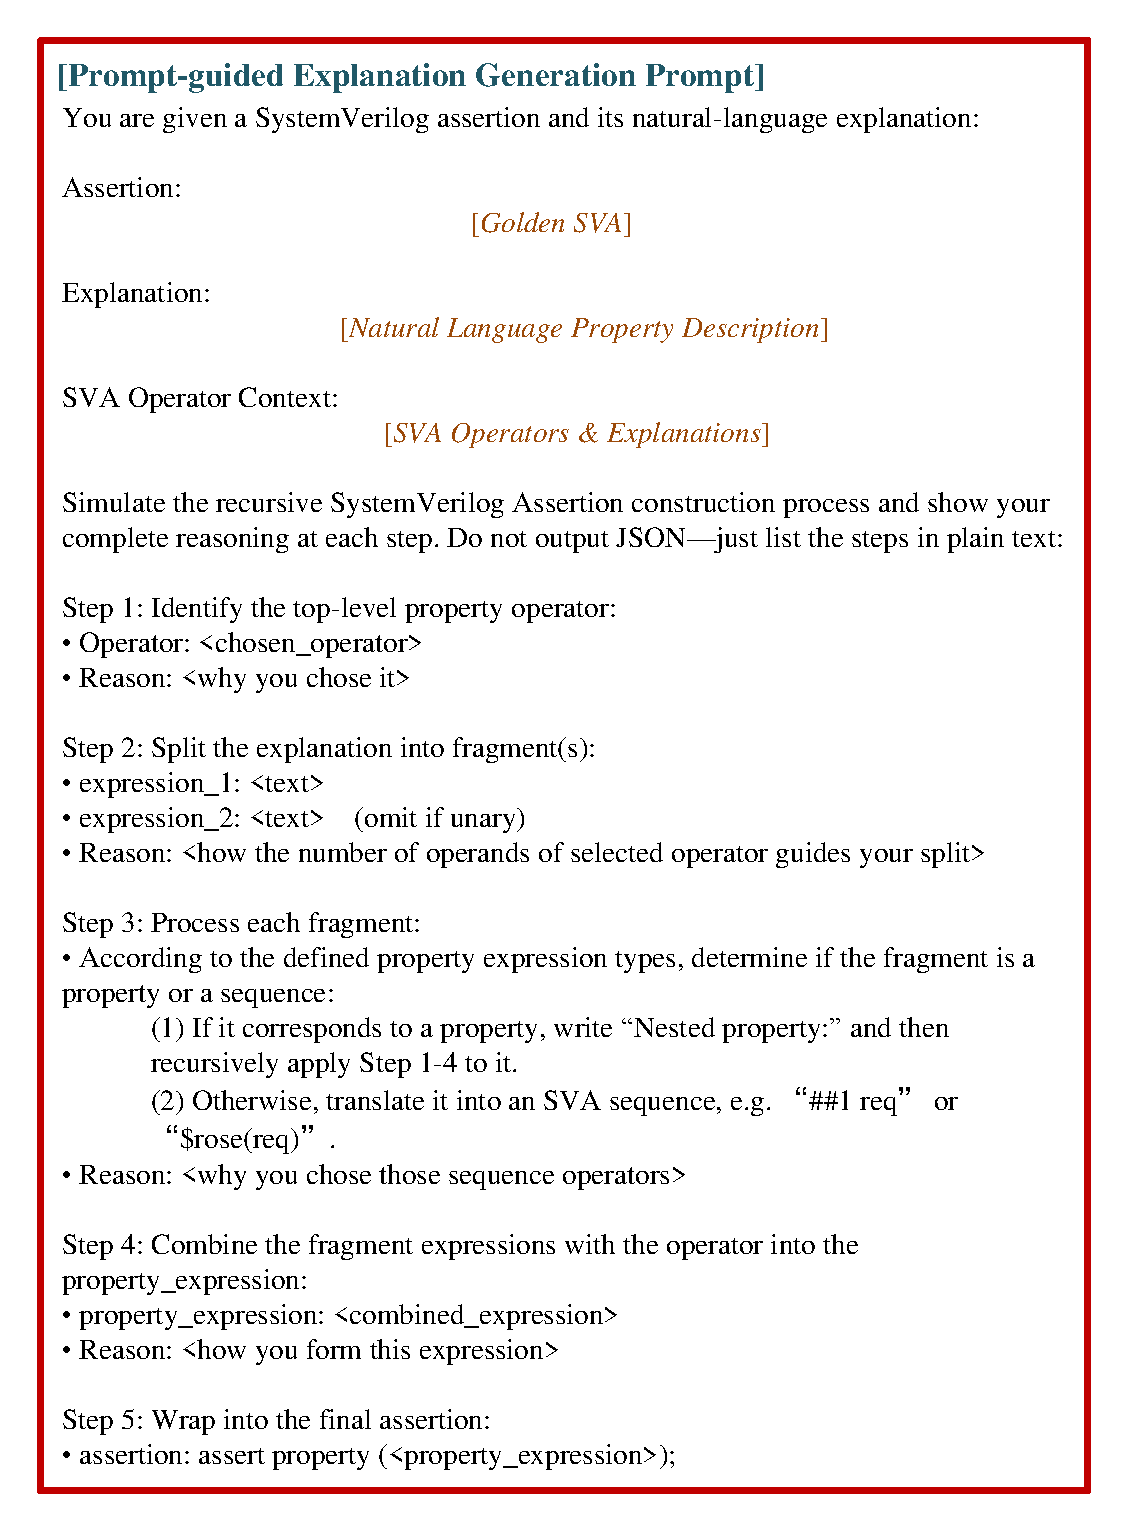
\includegraphics[width=0.6\linewidth]{Figs/Prompt-guided-Explanation-Generation.pdf}
    \caption{Prompt for generating the prompt-guided explanation.}
    \label{fig:prompt-guided-explanation-generation}
\end{figure}

\subsection{Example Prompt-guided Explanation}
\label{subsec:example-prompt-guided-explanation}
Golden SVA:
\begin{verbatim}
    @(posedge pclk) refSig |-> $stable(StableSig)
\end{verbatim}
Natural language explanation:

A property expression that for every rising edge of the clock at which a given reference signal \texttt{refSig} is true, the stable‐value check on another signal \texttt{StableSig} succeeds in that same cycle.
\\
\\
The corresponding prompt-guided explanation is shown in Fig.~\ref{fig:example-prompt-guided-explanation}, which is generated by OpenAI o4-mini.
\begin{figure}
    \centering
    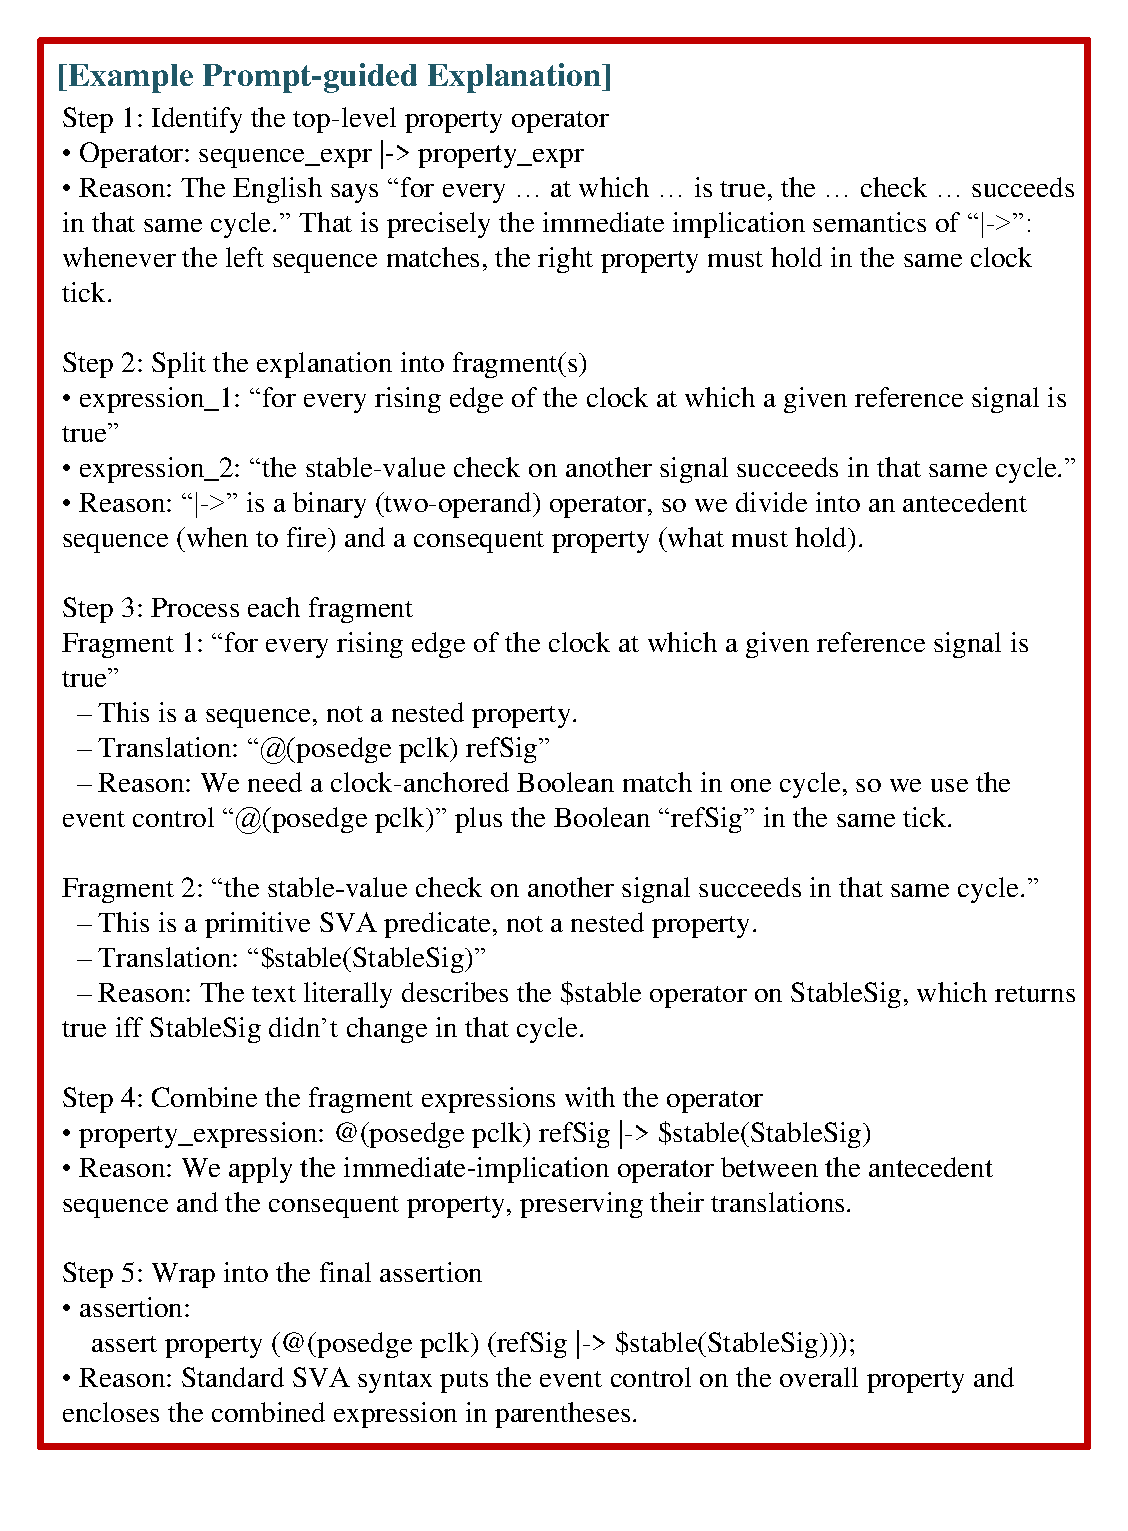
\includegraphics[width=0.6\linewidth]{Figs/Example-Prompt-Guided-Explanation.pdf}
    \caption{An example prompt-guided explanation.}
    \label{fig:example-prompt-guided-explanation}
\end{figure}



